\documentclass[oneside,final,14pt]{extreport}

\usepackage[T2A]{fontenc}
\usepackage[utf8]{inputenc}
\usepackage[russian]{babel}
\usepackage{vmargin}
\usepackage{../title_variables}
\usepackage{../../_styles/sourceCode}
\usepackage{../../_styles/tableOfContent}
\usepackage{../../_styles/hyperlinks}
\usepackage{../../_styles/Verbatim}

\setmarginsrb{10mm}{10mm}{10mm}{10mm}{0pt}{0mm}{0pt}{0mm}
\pagestyle{empty}
\begin{document}
    \begin{center}
    Министерство образования Республики Беларусь

    Учреждение образования

    <<Брестский государственный технический университет>>

    Кафедра \titlePageKafedra
\end{center}

\vfill

\begin{center}
    \titlePageTypeWork

    за \titlePageSemestr~семестр

    по дисциплине: {\bfseries \titlePageSubject}

    Тема: \titlePageTopic
\end{center}

\vfill

\begin{flushright}
    \begin{minipage}[tl]{7cm}
        \textbf{Выполнил}

        \smallskip

        \titlePageStudentType

        \titlePageStudentSurname~\titlePageStudentName

        \bigskip

        \textbf{Проверил}

        \smallskip

        \titlePageTeacherSurname~\titlePageTeacherName
    \end{minipage}
\end{flushright}

\vfill

\begin{center}
    \titlePageCity~\the\year{}
\end{center}

    \newpage
    \paragraph{Цель работы}
Создать UML диаграмму предметной области по варианту (Фабрика).


\paragraph{Задание}
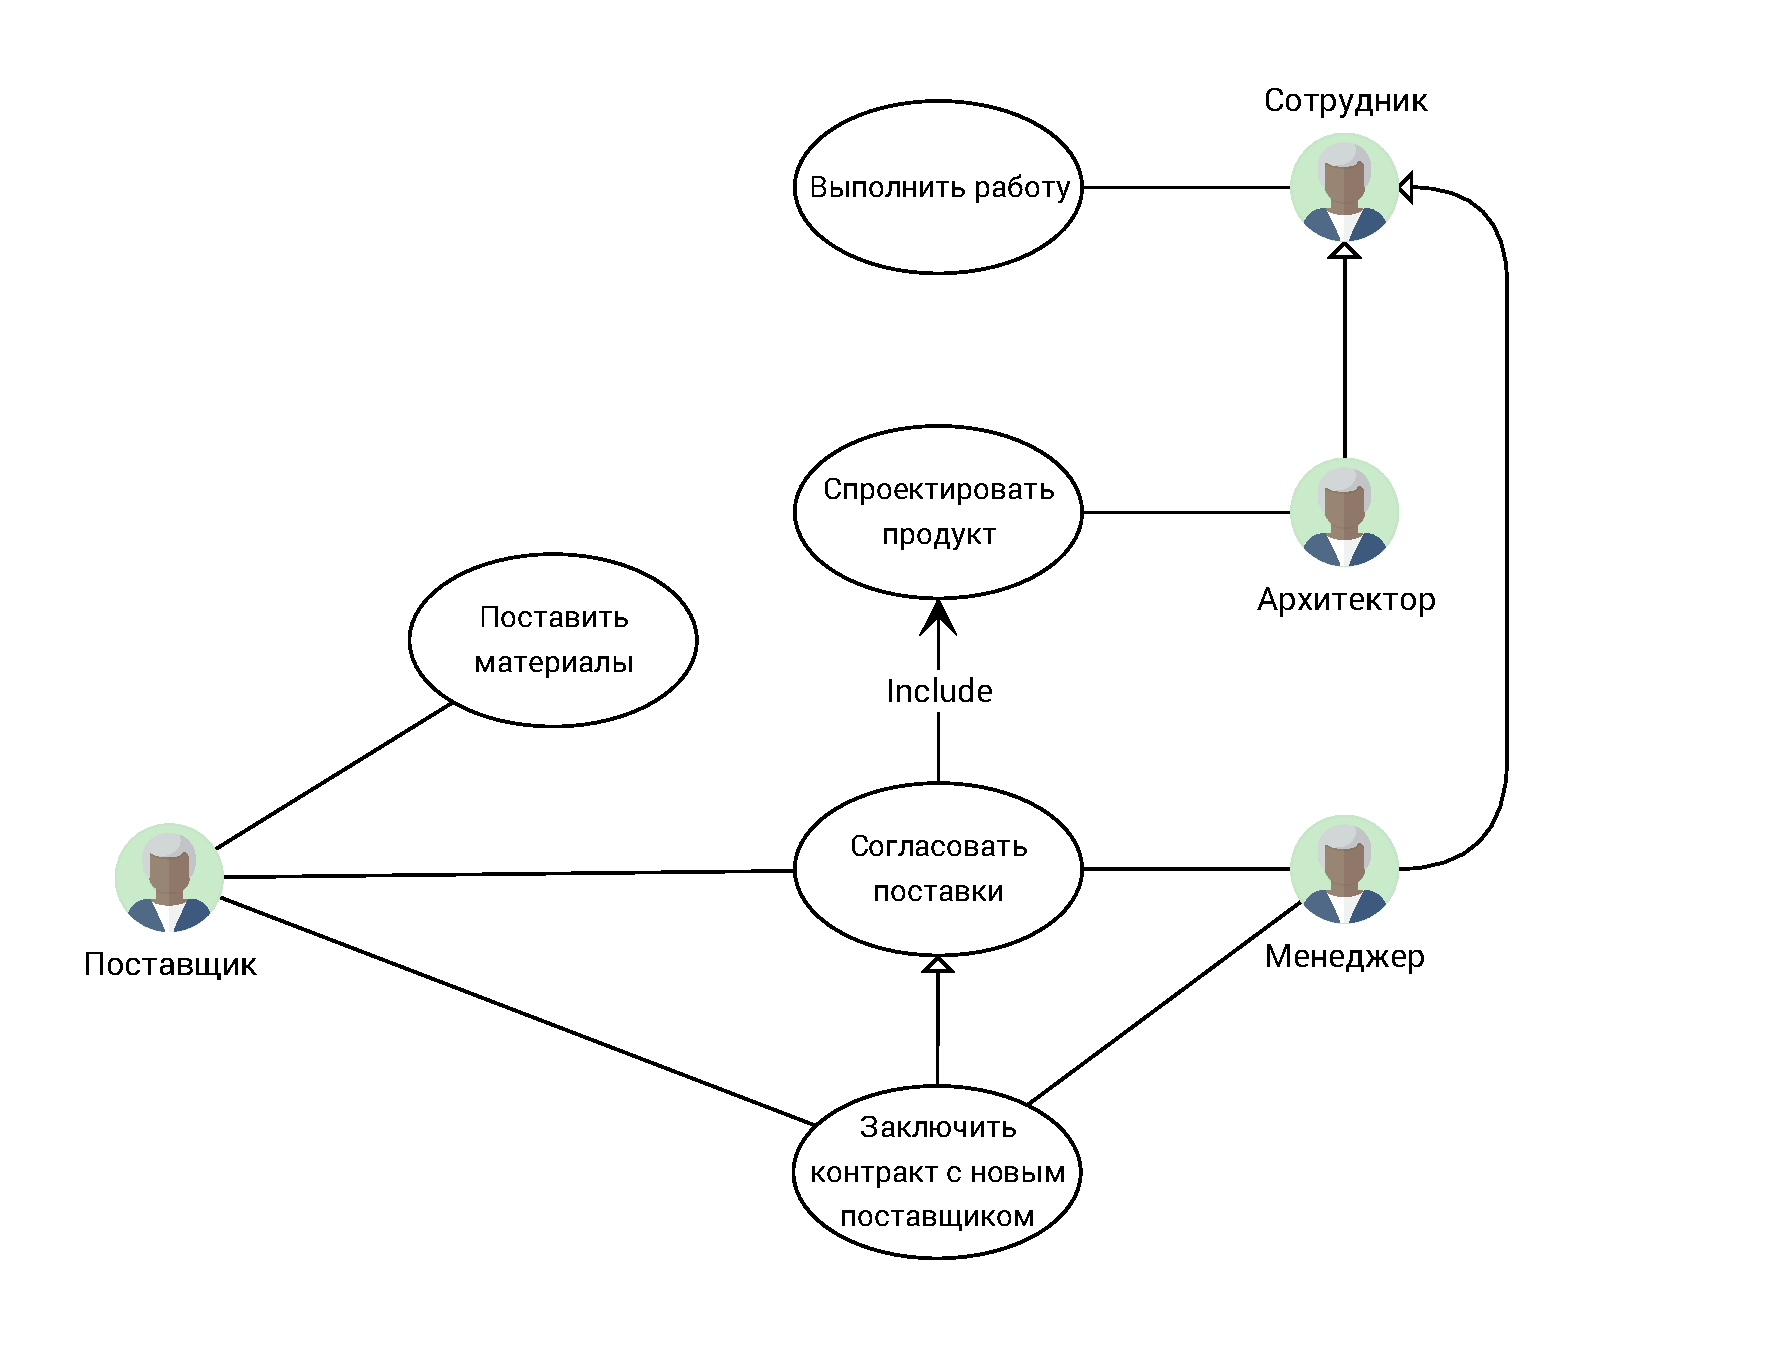
\includegraphics[width=0.9\textwidth]{social-network.pdf}

    \paragraph{Часть 2}
\subparagraph{Задание 1}

Изучите при помощи man опцию -l команды ls. Просмотрите права каталогов
/etc, /bin и домашнего каталога. Просмотрите права файлов, содержащиеся в этих
каталогов. Выявите тенденции (файлов с какими правами в каких каталогах больше).
Сделайте вывод.

\begin{verbatim}
ivan@pc:~/lab$ ls ~ -l
total 76
drwxrwxr-x  2 ivan ivan 4096 Jan 22 17:14 books
drwxrwxr-x  4 ivan ivan 4096 Jan 18 11:17 CLionProjects
drwxrwxr-x  3 ivan ivan 4096 Mar  5 19:24 configuration
drwxr-xr-x  2 ivan ivan 4096 Jan  3 02:32 Desktop
drwxr-xr-x  2 ivan ivan 4096 Feb 26 15:09 Documents
drwxr-xr-x 13 ivan ivan 4096 Mar  7 17:12 Downloads
drwxrwxr-x  3 ivan ivan 4096 Jan 10 22:05 external
drwxrwxr-x 11 ivan ivan 4096 Feb 26 22:45 IdeaProjects

-rwxr-xr-x 1 root root       216256 Apr 22  2017  zip
-rwxr-xr-x 1 root root        93816 Apr 22  2017  zipcloak
-rwxr-xr-x 1 root root        50718 Oct 19 13:56  zipdetails
-rwxr-xr-x 1 root root         2953 Aug 16  2019  zipgrep
-rwxr-xr-x 1 root root       186664 Aug 16  2019  zipinfo
-rwxr-xr-x 1 root root        89488 Apr 22  2017  zipnote
-rwxr-xr-x 1 root root        93584 Apr 22  2017  zipsplit
-rwxr-xr-x 1 root root        26952 Jan 30  2020  zjsdecode
-rwxr-xr-x 1 root root         2206 Dec 13  2019  zless
-rwxr-xr-x 1 root root         1842 Dec 13  2019  zmore
-rwxr-xr-x 1 root root         4553 Dec 13  2019  znew
\end{verbatim}

В домашнем каталоге владелец я, к корневом --- root.

\subparagraph{Задание 2}
Изучите материал, посвящѐнный пользователям и группам пользователей.
Изучите руководство по командам chown и chgrp. Выясните, кто является владельцем и
к какой группе владельцов принадлежат файлы вашего домашнего каталога, каталогов
/etc, /root, /bin и /dev.

chown и chgrp позволяют менять владельца и группу файлов.
В /home владелец всегда я.
В /root я не могу получить доступ без использования sudo.
В /etc, /bin, /dev владелец чаще root, но иногда video, disk, tty.

\subparagraph{Задание 3}
Определите атрибуты файлов /etc/shadow и /etc/passwd попробуйте вывести на
экран содержимое этих файлов. Объясните результат.
\begin{verbatim}
ivan@pc:~/lab$ ls -l /etc/shadow
-rw-r----- 1 root shadow 1504 Feb  5 23:12 /etc/shadow

ivan@pc:~/lab$ ls -l /etc/passwd
-rw-r--r-- 1 root root 2881 Feb  5 23:12 /etc/passwd
\end{verbatim}
Файлы связаны с безопасностью, поэтому прав почти нет.

\subparagraph{Задание 4}
Изучите команду chmod. Создайте в домашнем каталоге любые четыре файла,
установите при помощи восьмеричных масок на каждый из них в отдельности
следующие права:

- для себя все права, для группы и остальных - никаких;

- для себя чтение и запись, для группы чтение, для остальных - все;

- для себя исполнение и запись, для группы никаких, для остальных чтение;

- для себя запись, для группы все, для остальных - только запись.
\begin{verbatim}
ivan@pc:~/lab$ chmod 647 1
ivan@pc:~/lab$ chmod 700 1
ivan@pc:~/lab$ chmod 647 2
ivan@pc:~/lab$ chmod 306 3
ivan@pc:~/lab$ chmod 272 4
ivan@pc:~/lab$ ls -l
total 0
-rwx------ 1 ivan ivan 0 Mar  7 21:31 1
-rw-r--rwx 1 ivan ivan 0 Mar  7 21:31 2
--wx---rw- 1 ivan ivan 0 Mar  7 21:31 3
--w-rwx-w- 1 ivan ivan 0 Mar  7 21:31 4
\end{verbatim}

Используя лишь символы
\begin{verbatim}
ivan@pc:~/lab$ ls -l
total 0
---------- 1 ivan ivan 0 Mar  7 21:31 1
---------- 1 ivan ivan 0 Mar  7 21:31 2
---------- 1 ivan ivan 0 Mar  7 21:31 3
---------- 1 ivan ivan 0 Mar  7 21:31 4
ivan@pc:~/lab$ chmod u+rwx
chmod: missing operand after ‘u+rwx’
Try 'chmod --help' for more information.
ivan@pc:~/lab$ chmod u+rwx 1
ivan@pc:~/lab$ chmod u+rw 2
ivan@pc:~/lab$ chmod g+r 2
ivan@pc:~/lab$ chmod o+rwx 2
ivan@pc:~/lab$ chmod u+wx 3
ivan@pc:~/lab$ chmod o+w 3
ivan@pc:~/lab$ chmod u+w 4
ivan@pc:~/lab$ chmod g+rwx 4
ivan@pc:~/lab$ chmod o+w 4
ivan@pc:~/lab$ ls -l
total 0
-rwx------ 1 ivan ivan 0 Mar  7 21:31 1
-rw-r--rwx 1 ivan ivan 0 Mar  7 21:31 2
--wx----w- 1 ivan ivan 0 Mar  7 21:31 3
--w-rwx-w- 1 ivan ivan 0 Mar  7 21:31 4    
\end{verbatim}

\subparagraph{Задание 4}

В домашнем каталоге создайте файл и установите на него права так, чтобы его
можно было только редактировать.

\begin{verbatim}
ivan@pc:~/lab$ touch file
ivan@pc:~/lab$ chmod 666 file
\end{verbatim}

\subparagraph{Задание 5}
Скопируйте в свой домашний каталог файл ls из каталога /bin. Запретите
выполнение этого файла и попробуйте выполнить именно его, а не исходный(!).
Объясните результат.
\begin{verbatim}
ivan@pc:~/lab$ cp /bin/ls ls20
ivan@pc:~/lab$ chmod a-x ls20
ivan@pc:~/lab$ ./ls20
bash: ./ls20: Permission denied
\end{verbatim}
    \subparagraph{Вывод}
    Я познакомился с правами доступа в Linux, способами их изменения, а также узнал, какие типы владения существуют.
    Разобрался с символьными и жёсткими ссылками.
\end{document}
